\documentclass[11pt,a4paper,twocolumn,twoside]{paper}
\usepackage[utf8]{inputenc}
\usepackage{amsmath}
\usepackage{amsfonts}
\usepackage{amssymb}
\usepackage{graphicx}
\usepackage{listings}
\usepackage{wrapfig}
\usepackage{enumitem}
\usepackage{helvet}
\usepackage{tikz}
\usepackage[most]{tcolorbox} % pacchetto per box colorate
\usepackage{xcolor} % colori personalizzati
\usepackage{caption}
\usepackage{listings}
\usetikzlibrary{arrows,automata,positioning}
\lstset{
  language=Bash,
  basicstyle=\ttfamily\small,
  keywordstyle=\color{blue},
  commentstyle=\color{gray},
  stringstyle=\color{orange},
  numbers=left,
  numberstyle=\tiny,
  stepnumber=1,
  frame=single,
  breaklines=true
}
\renewcommand{\familydefault}{\sfdefault}
\usepackage[left=1cm, right=1cm, top=3cm, bottom=2cm]{geometry}
\author{Luca Serafini (672707)}
\title{\vspace{-6em}Documentazione Progetto Reti Informatiche\\Ingegneria Informatica UNIPI A.A. 25/26 (DISPARI)}
\subtitle{\today}
\begin{document}
\maketitle
\paragraph{Descrizione}
    \textbf{Kanban} è un'applicazione utilizzata per gestire una lavagna Kanban e gli utenti associati ad essa. L'applicazione presenta un'architettura ibrida: di tipo \textit{Client-Server} per il collegamento tra utente e lavagna, data la necessità per gli utenti di riferirsi ad un unico dispositivo per la gestione delle card; \textit{Peer-to-Peer} per il collegamento tra utenti, che si inviano messaggi sporadici per la revisione dei loro job. 
\paragraph{Struttura del progetto}
    Il progetto è suddiviso in varie cartelle: la cartella class è condivisa tra lavagna e utenti, contiene strutture dati e funzioni relative ad esse; vi è poi il file structs/enums.h che contiene tipi enumerati e macro; network per implementare funzionalità di rete; functions e server, cartelle che implementano funzionalità relative alla sola lavagna e user, che contiene le funzioni relative all'utente.  
\paragraph{Lavagna}
    La \textbf{lavagna} è l'elemento centrale dell'architettura. Essa sfrutta l'IO-multiplexing, tramite la chiamata di sistema \textit{select}, per rimanere in ascolto di:
    \begin{itemize}
        \item \textit{Socket} TCP degli utenti
        \item Una pipe, utilizzata per la gestione del timer
    \end{itemize}
    Essendo l'applicazione a comunicazione asincrona, e supponendo un numero ridotto di utenti\footnote{Si presuppone che gli utilizzatori di questa applicazione siano team di dimensioni modeste}, ho scelto di utilizzare la \textit{select}, con un solo thread, dato che le singole operazioni sono molto rapide, e non richiedono elevati tempi di computazione. Nonostante una soluzione multi-thread possa risultare più rapida, dato il tipo di applicazione non è necessaria una velocità così elevata, ed è quindi più conveniente utilizzare la soluzione single-thread, evitando possibili errori nell'implementazione della \textit{mutua esclusione}. Una volta ricevuto un segnale dall'utente, si verifica se sia un tentativo di connessione o un messaggio socket\footnote{Un messaggio che arriva alla select da un utente è sempre un comando}: nel primo caso si verifica che non esista un altro utente con lo stesso numero di porta, in tal caso si crea l'utente e gli si fornisce la card; nel secondo si passa il comando alla funzione \textit{handle\_message}, che esegue le operazioni necessarie. Il server utilizza una struttura dati di tipo \textbf{Board} per gestire gli utenti connessi e le card.
\paragraph{Timer}
    Non essendo specificato nella richiesta, ho ritenuto che se un utente non risponde con ACK\_CARD ad una HANDLE\_CARD del server per più di 120 secondi, esso viene considerato inattivo e conseguentemente disconnesso. Per l'implementazione di questa funzionalità, quella della PING\_LAVAGNA e quella di disconnessione dell'utente alla mancata PONG\_LAVAGNA, ho creato una struttura dati Timer\_s, ovvero una lista che ad ogni elemento contiene: una funzione e il suo argomento (porta dell'utente), la porta dell'utente e il timestamp a cui dev'essere eseguita. L'inserimento degli elementi nel timer avviene sempre in ordine di timestamp, in modo tale che gli eventi più vicini siano in testa. Successivamente si chiama la \textit{alarm} sul tempo che intercorre il timestamp attuale e l'elemento in testa della lista, al termine del quale viene segnalata alla select che una funzione è pronta per essere eseguita (scrivendo un valore su una pipe attenzionata dalla select), il quale la eseguirà, e nel caso vi siano altri elementi in lista, verrà chiamata un alarm sull'elemento in testa. L’uso di \textit{alarm} è adeguato data la presenza di un singolo thread e di un solo flusso di gestione degli eventi temporali.

    \begin{figure}[h!] % [h!] cerca di posizionare la figura "qui"
    \centering
    % Spaziatura verticale extra sopra la figura (opzionale)
    \vspace{0.1cm} 
    
    % fbox crea il bordo nero attorno al contenuto
    \fbox{
        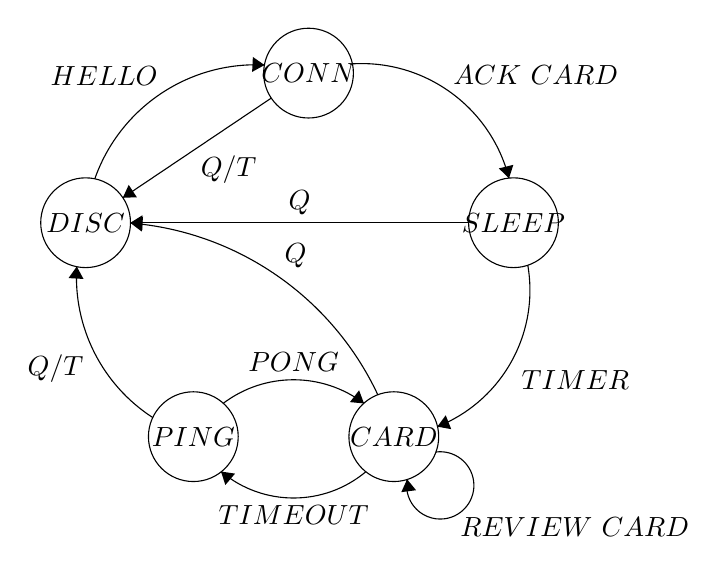
\begin{tikzpicture}[scale=0.19]
            \tikzstyle{every node}+=[inner sep=0pt]
            \draw [black] (21.3,-5.7) circle (3);
            \draw (21.3,-5.7) node {$CONN$};
            \draw [black] (35,-15.7) circle (3);
            \draw (35,-15.7) node {$SLEEP$};
            \draw [black] (13.6,-30) circle (3);
            \draw (13.6,-30) node {$PING$};
            \draw [black] (6.4,-15.7) circle (3);
            \draw (6.4,-15.7) node {$DISC$};
            \draw [black] (27,-30) circle (3);
            \draw (27,-30) node {$CARD$};
            \draw [black] (7.013,-12.772) arc (160.64338:87.09098:11.411);
            \fill [black] (18.36,-5.16) -- (17.58,-4.62) -- (17.53,-5.62);
            \draw (7.64,-6.58) node [above] {$HELLO$};
            \draw [black] (18.81,-7.37) -- (8.89,-14.03);
            \fill [black] (8.89,-14.03) -- (9.83,-14) -- (9.28,-13.17);
            \draw (15.96,-11.2) node [below] {$Q/T$};
            \draw [black] (24.224,-5.081) arc (93.49653:14.25004:10.167);
            \fill [black] (34.7,-12.73) -- (34.99,-11.83) -- (34.02,-12.07);
            \draw (36.48,-6.52) node [above] {$ACK\mbox{ }CARD$};
            \draw [black] (25.145,-32.333) arc (-49.91384:-130.08616:7.524);
            \fill [black] (15.45,-32.33) -- (15.74,-33.23) -- (16.39,-32.47);
            \draw (20.3,-34.6) node [below] {$TIMEOUT$};
            \draw [black] (35.954,-18.532) arc (9.85724:-68.30608:9.814);
            \fill [black] (29.91,-29.33) -- (30.84,-29.5) -- (30.47,-28.57);
            \draw (35.51,-26.21) node [right] {$TIMER$};
            \draw [black] (10.893,-28.727) arc (-122.88022:-183.66959:11.169);
            \fill [black] (5.81,-18.63) -- (5.26,-19.4) -- (6.26,-19.46);
            \draw (6.29,-25.48) node [left] {$Q/T$};
            \draw [black] (32,-15.7) -- (9.4,-15.7);
            \fill [black] (9.4,-15.7) -- (10.2,-16.2) -- (10.2,-15.2);
            \draw (20.7,-15.2) node [above] {$Q$};
            \draw [black] (15.589,-27.779) arc (127.14833:52.85167:7.802);
            \fill [black] (25.01,-27.78) -- (24.68,-26.9) -- (24.07,-27.69);
            \draw (20.3,-25.7) node [above] {$PONG$};
            \draw [black] (9.397,-15.722) arc (85.30759:25.1576:20.083);
            \fill [black] (9.4,-15.72) -- (10.15,-16.29) -- (10.24,-15.29);
            \draw (20.43,-18.74) node [above] {$Q$};
            \draw [black] (29.806,-31.028) arc (97.60282:-190.39718:2.25);
            \draw (39.09,-35.37) node [below] {$REVIEW\mbox{ }CARD$};
            \fill [black] (27.89,-32.85) -- (27.5,-33.71) -- (28.49,-33.58);
        \end{tikzpicture}
    } % Chiusura fbox
    
    % Didascalia e Label
    \caption{Automa a stati finiti (FSM) dell'Utente}
    \label{fig:automa_utente}
\end{figure}
\paragraph{Utenti} 
    Gli utenti rappresentano i vari client del progetto. Gli utenti possono essere definiti tramite un automa a stati finiti (Fig. 1). Nel mio caso ho implementato questo concetto tramite l'ausilio del tipo enumerato \textbf{User\_status} (\textit{enums.h}). Esso identifica lo stato corrente dell'utente, e in base a ciò viene permesso o meno all'utente di avviare date funzioni in base allo stato. Per gestire l'utente vengono utilizzate due variabili: \textbf{user\_data} e \textbf{review}. La prima contiene tutte le informazioni necessarie relative all'utente: stato in cui si trova, carta che sta gestendo, porte e socket della lavagna e degli altri peer. La seconda, invece, viene utilizzata durante il processo di review, e contiene un array con gli utenti che devono ancora revisionare la propria card. L'utente utilizza una select in ascolto del socket TCP con la lavagna, UDP con gli altri utenti e una pipe per gli eventi del timer. Per simulare lo svolgimento della card, si utilizza un altro thread, che chiama la sleep per un tempo casuale compreso tra i 10 e i 30 secondi.
\paragraph{Comunicazione Utente-Lavagna}
    La comunicazione tra utente e lavagna avviene tramite un socket TCP, seguendo il paradigma Client-Server, dato che l'utente si registra fisicamente alla lavagna e invia spesso comandi. I comandi e i dati passati, devono arrivare tutti integri, per questo ho scelto un protocollo di comunicazione affidabile.
\paragraph{Comunicazione tra utenti}
     La comunicazione tra utenti avviene tramite un socket UDP. Ogni utente è in ascolto del suo socket, e invia messaggi agli altri, sapendo che il loro socket si trova alla porta da loro specificata come ID. La comunicazione Peer-to-Peer avviene esclusivamente per la revisione di card, per questo utilizzo il protocollo non affidabile: essendo una sorta di "notifica", non è necessario che gli utenti siano tutti connessi\footnote{Questo implica anche meno tunnel TCP da gestire}. Per questa funzionalità ho deciso di utilizzare questo paradigma, poiché riflette la natura logica dell'operazione: mentre la Lavagna rappresenta l'autorità centrale per la persistenza dei dati, la revisione è un'interazione diretta e transitoria tra due pari. La revisione avviene tramite l'invio del comando \textbf{REVIEW\_CARD}, con il quale si invia agli altri utenti attivi una notifica relativa all'utente che richiede la revisione. Nel frattempo viene avviato un timer di 30 secondi. Agli utenti che devono revisionare viene aggiunto un comando \textbf{REVIEW}, tramite il quale possono revisionare il task dell'utente che hanno ricevuto per primo\footnote{Dato che possono essere inviati più task da più utenti diversi, i successivi possono essere revisionati in ordine FCFS}. Nel caso in cui il messaggio UDP o la notifica di revisione non arrivasse all'altro host, il timer, ogni 30 secondi, controlla gli utenti della lavagna rimasti (se ne sono stati rimossi alcuni, essi verranno rimossi anche dalla struttura "review", nel caso ne venissero aggiunti altri rispetto allo stato iniziale, essi non revisioneranno la card), inviandogli un'altra notifica.
    
\paragraph{Protocolli di invio dei messaggi}
    Per inviare i messaggi ho scelto di utilizzare sia protocolli text che binary. Distinguiamo le principali macro-categorie di messaggi:
    \begin{itemize}
        \item I \textbf{comandi TCP}, ovvero quelli tra lavagna e utente, sono gestiti tramite due strutture di tipo enumerato, Board\_to\_User\_command (per inviare messaggi dalla lavagna all'utente) e User\_to\_Board\_command (per l'operazione inversa). La scelta ricade quindi sul protocollo binary. Questa scelta garantisce efficienza (dimensione del pacchetto fissa e ridotta) e scalabilità, permettendo l'aggiunta di nuove funzionalità semplicemente estendendo la definizione dell'enumerato, senza modificare la logica di parsing di basso livello.
        \item I \textbf{comandi UDP}, ovvero quelli che vengono inviati tra utenti, utilizzano anch'essi il protocollo binary, dato che ho bisogno di una struttura ben definita che mi specifichi porta dell'utente trasmettitore e carta che deve essere revisionata (o -1, nel caso di messaggio di revisione)\footnote{L'uso di una struct a dimensione fissa evita l'overhead di parsing complesso.}.
        \item Il resto dei messaggi varia: per inviare i numeri utilizzo il protocollo binario; le \textbf{stringhe di testo}, invece, vengono inviate precedute da un intero che ne indica la dimensione esatta. Questo permette al ricevente di allocare dinamicamente il buffer corretto e leggere esattamente i byte necessari, evitando le ambiguità tipiche dei protocolli puramente testuali basati su delimitatori. 
    \end{itemize}
\paragraph{Istruzioni di compilazione}
    Per compilare i file è sufficiente utilizzare il comando
    \begin{lstlisting}
make
    \end{lstlisting}
\end{document}
